\section{Economic Analysis}\label{sec:economy}
\phantomsection

\subsection{Project description}
This section covers the analysis of the developed product from an economic point of view. This product is a web application which whose aim is to facilitate the process of automatically taking long term time-lapses with DSLR Cameras. This section describes aspects like the usefulness of the product, market research, project and time schedule as well as the profitability of the implemented solution.

\subsection{Project time schedule}
The success of the project depends on the right establishing of time constrains of involved activities
as well as resources involved in those activities. For the accomplishment of a project it is necessary to establish a schedule. For the development of the DSLR Camera Controller application, Agile project management is applied to offer flexible and iterative method of designing the application. It goes in 6 stages: requirements, design, develop, test, deploy and feedback. These steps are represented in the figure \mbox{\ref{agile}}. It is a set of repetitive actions which were proven to have a substantial effect on the development of a product.

\begin{figure}[!ht]
\centering
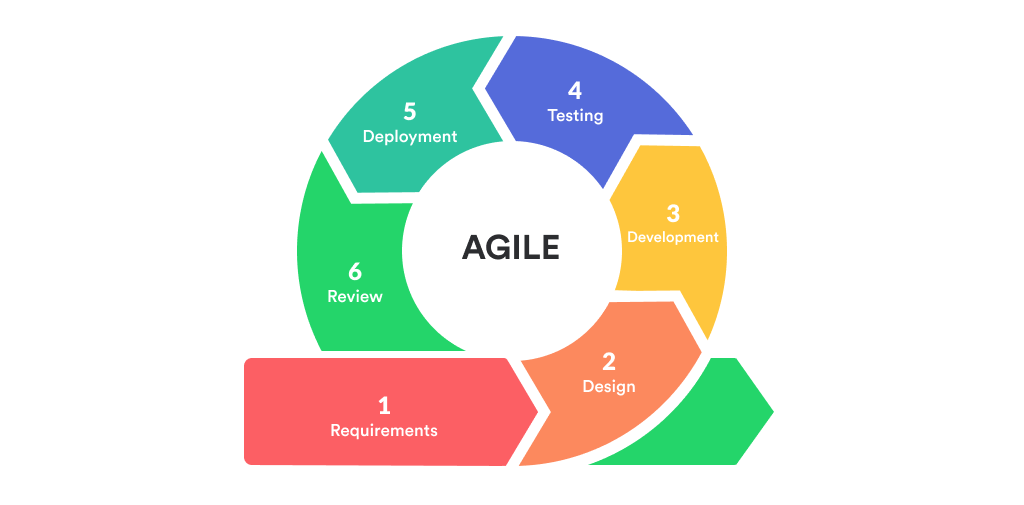
\includegraphics[width=15cm]{4-agile-chart}
\caption{Agile development}\label{agile}
\end{figure}

\subsubsection{Objective determination}
The main objective of the following project is to provide a complete and functioning application for photographers. Otherwise without a finished product there can be no profit. More to that, it is important to market the application and get exposed to a large audience in need. This can be done by targeting first the company that has originally proposed this project.

As it was originally a project requested by the photographic department of CERN (the European Organization for Nuclear Research), this company will prove to be the best first target. Additionally, CERN is still struggling with the automation of taking photos in general, so it can prove to be a client that may offer other projects in the same field in the future. For example, there's a problem in automation of the process of generating a 3D model for VR of the Large Hadron Collider. A project was proposed to create a robot which would take photos of the entire accelerator, then through photographic technologies generate a 3D model. Considering the similarities, it is a project worth considering for future development.

\subsubsection{Time schedule establishment}
Time management is an important factor in determining the success of a product. So, as mentioned above, the project will iterate over 6 steps every sprint. Because the required team is not very big, to enure the maximum performance, the sprints will be divided into one week each. Naturally, the first few sprints will be mostly composed of research tasks, to analyze the available tools currently available. But normally the sprint will start by deciding on a set of stories that the team should manage to finish until the end of the week. This includes the requirements and design stages. Next follows the development stage followed by the testing stage. Once the stories are finished, they are tested on a development environment. Depending on how successful was the testing part, the application is then deployed on a staging environment where the client can interact with the application and leave feedback. Additionally, the team will also make brief morning Standups just to ensure that everyone is on the same page. Depending on how well the team performs, new ceremonies like sprint review and sprint retrospective can be done once in a while. Total duration of the project is computed using \eqref{eq:duration}.

\begin{equation} \label{eq:duration}
 D_T = D_F - D_S + T_R,
\end{equation}
\noindent

where $D_T$ is the duration, $D_F$ -- the finish date, $D_S$ -- the start date and $T_R$ -- reserve time. In table \ref{table:schedule} is presented the first iteration of the project schedule. It uses the following notations:
\begin{itemize}
   \item PM -- project manager
   \item SA -- system architect
   \item SM -- sales manager
   \item D -- developer
\end{itemize}

\begin{table}[!ht]
\begin{center}
\caption{Time schedule}
\renewcommand{\arraystretch}{2}
\begin{tabular}{| c | >{\centering\arraybackslash}p{5cm} | >{\centering\arraybackslash}p{2cm} | c | >{\centering\arraybackslash}p{5cm} |}
\hline
\textbf{Nr} & \textbf{Activity Name} & \textbf{Duration (days)} & \textbf{People involved} & \textbf{Comments} \\
\hline
1 & Define the project concept and objectives & 5 & PM, SA, SM, D & It is a common task \\
\hline
2 & Perform market analysis & 10 & PM, SA & Will results into a document describing market analysis \\
\hline
3 & Analysis of the domain & 15 & SA, D & Research of the recognition algorithms \\
\hline
4 & Write down requirements and specifications & 5 & PM, SA, D & \\
\hline
5 & System design (UML) & 10 & PM, SA, D & \\
\hline
6 & Database design & 5 & PM, SA, D & Development database and end-user database schemes\\
\hline
7 & Preprocessing and learning part of the implementation & 30 & PM, SA, D & \\
\hline
8 & End-user application development & 20 & PM, SA, D, SM & \\
\hline
9 & Validation of results & 10 & PM, SA, D, SM & \\
\hline
10 & Documentation & 5 & D & \\
\hline
11 & Deployment and testing & 10 & PM, SA, D & \\
\hline
12 & Active marketing & 10 & SM & \\
\hline
13 & Total time to finish the system & 135 & & \\
\hline
\end{tabular}
\label{table:schedule}
\vspace{-2.5em}
\end{center}
\end{table}

Table \ref{table:schedule} describes the activities that will occur during project development, who is involved into each process and how much time does it take to accomplish a task. Total amount of time spent on the following project is estimated to be 135 days.

\subsection{Economic motivation}
The following section describes the evaluation of the project from the economic point of view. That includes the total profit, number of potential clients, salaries that have to be paid to employees, revenues that the company gets by commercializing the product. All the costs and prices are given in MDL (Moldavian lei) currency. Tangible and intangible assets, indirect expenses will also be taken into account. Wear and depression in regard to final product will also be computed. It should be mentioned that DSLR Camera Controller is an open source project posted publicly on Github. In production and development, open source as a development model promotes a universal access via a free license to a product's design or blueprint, and universal redistribution of that design or blueprint, including subsequent improvements to it by anyone. Before the phrase "open source" became widely adopted, developers and producers used a variety of other terms. Open source gained hold with the rise of the Internet, and the attendant need for massive retooling of the computing source code. Opening the source code enabled a self-enhancing diversity of production models, communication paths, and interactive communities. The open-source software movement arose to clarify the environment that the new copyright, licensing, domain, and consumer issues created. The entire economical part is done on the presumption that the software will have payed licenses. Either way it is a curios approach to compute all the necessary resources and indexes for developing a project. It opens managerial insights over entrepreneurial ideas.

\subsubsection{Tangible and intangible asset expenses}
The budget of a project is most of the times what shapes the future development process. Depending on the budget, some additional features can be implemented or otherwise, can be dropped because of insufficient funding. In this section, the budget will be defined and computed so that managing it would be easier in the future. In \mbox{Table \ref{table:tangible_assets}} are presented all the tangible assets used for developing this product. Tangible assets are defined as a set of assets that have a physical form.

\begin{table}[!hb]
\begin{center}
\caption{Tangible asset expenses}
\renewcommand{\arraystretch}{2}
\begin{tabular}{| c | c | >{\centering\arraybackslash}p{2.7cm} | >{\centering\arraybackslash}p{2cm} | c | >{\centering\arraybackslash}p{5em}|}
\hline
\textbf{Material} & \textbf{Specification} & \textbf{Measurement unit} & \textbf{Price per unit (MDL)} & \textbf{Quantity} & \textbf{Sum (MDL)}\\
\hline

Mac Book pro & retina display i5 & Unit & 23000 & 1 &  \multicolumn{1}{r|}{23000}\\
\hline

Camera & Sony Alpha-A3000 & Unit & 8000 & 1 & \multicolumn{1}{r|}{8000}\\
\hline

Camera & Nikon Z6 & Unit & 32000 & 1 & \multicolumn{1}{r|}{8000}\\
\hline

\multicolumn{5}{|r|}{Total} & \multicolumn{1}{r|}{63000}\\
\hline
\end{tabular}
\label{table:tangible_assets}
\end{center}
\vspace{-1.3em}
\end{table}

The opposite of tangible assets are intangible assets, which are considered nonphysical investments. These assets are presented in the \mbox{Table \ref{table:intangible_assets}}.

\begin{table}[!hb]
\begin{center}
\caption{Intangible asset expenses}
\renewcommand{\arraystretch}{2}
\begin{tabular}{| c | >{\centering\arraybackslash}p{5cm} | >{\centering\arraybackslash}p{2.7cm} | >{\centering\arraybackslash}p{2cm} | c | >{\centering\arraybackslash}p{5em}|}
\hline
\textbf{Material} & \textbf{Specification} & \textbf{Measurement unit} & \textbf{Price per unit (MDL)} & \textbf{Quantity} & \textbf{Sum (MDL)} \\
\hline

License & Enterprise Architect Desktop Edition License & Unit & 1900 & 3 & \multicolumn{1}{r|}{5700} \\
\hline

License & PyCharm Commercial License & Month & 160 & 5 & \multicolumn{1}{r|}{800}\\
\hline

\multicolumn{5}{|r|}{Total} & \multicolumn{1}{r|}{6500}\\
\hline
\end{tabular}
\label{table:intangible_assets}
\vspace{-1em}
\end{center}
\end{table}

Below, in \mbox{Table \ref{table:direct_expenses}} are presented the direct expenses which appeared during this project. These expenses appeared during project development and cannot be included in any of the previous tables, because their value can not be added directly into the budget.

\begin{table}[!hb]
\begin{center}
\caption{Direct expenses}
\renewcommand{\arraystretch}{2}
\begin{tabular}{| >{\centering\arraybackslash}p{5em} | >{\centering\arraybackslash}p{7em} | >{\centering\arraybackslash}p{7em} | >{\centering\arraybackslash}p{5em} | >{\centering\arraybackslash}p{5em} | r |}
\hline
\textbf{Material} & \textbf{Specification} & \textbf{Measurement unit} & \textbf{Price per unit (MDL)} & \textbf{Quantity} & \multicolumn{1}{>{\centering\arraybackslash}p{5em}|}{\textbf{Sum (MDL)}}\\
\hline
Whiteboard & Universal Dry Erase Board & Unit & 500 & 1 & 500 \\
\hline
Paper & A4 & 500 sheets & 60 & 2 & 120 \\
\hline
Marker & Whiteboard marker & Unit & 15 & 10 & 150 \\
\hline
Pen & Blue pen & Unit & 5 & 20 & 100 \\
\hline
\multicolumn{5}{|r|}{Total} & 870 \\
\hline
\end{tabular}
\label{table:direct_expenses}
\vspace{-1.5em}
\end{center}
\end{table}

So the total amount of direct expenses in MDL is

\begin{equation}
 T_{e} = 63000 + 6500 + 870 = 70370
\end{equation}

\subsubsection{Salary expenses}
This section is concerned about the salaries to employees and various funds that should be paid. The distribution of salaries is the following: project manager - 400MDL, system architect - 450 MDL, sales manager - 300 MDL, developer - 380 MDL. The \mbox{Table \ref{table:salaries}} presents more thoroughly what would be the expenses for paying the salaries.

\begin{table}[!ht]
\begin{center}
\caption{Salary expenses}
\renewcommand{\arraystretch}{2}
\begin{tabular}{| >{\centering\arraybackslash}p{8em} | >{\centering\arraybackslash}p{8em} | >{\centering\arraybackslash}p{8em} | r |}
\hline
\textbf{Employee} & \textbf{Work fund (days)} & \textbf{Salary per day (MDL)} & \multicolumn{1}{>{\centering\arraybackslash}p{5em}|}{\textbf{Salary fund (MDL)}}\\
\hline
Project Manager & 105 & 400 & 42000 \\
\hline 
System Architect & 110 & 450 & 49500\\
\hline
Sales Manager & 45 & 300 & 13500\\
\hline
Developer & 115 & 380 & 43700\\
\hline
\multicolumn{3}{|r|}{Total} & 148700\\
\hline
\end{tabular}
\label{table:salaries}
\vspace{-2.5em}
\end{center}
\end{table}

Now by having computed all the salaries for the employees, it is time to compute how much to be paid to social services fund, medical insurance fund and the total work expenses by summing up all previous expenses. 

This year the social service fund is approved to be $23\%$, therefore the salary expenses are computed according to the relation \eqref{eq:fs}.

\begin{equation}\label{eq:fs}
\begin{split}
 FS &= F_{re} \cdot T_{fs} \\
    &= 148700 \cdot 23 \% \\
    &= 34201,
\end{split}
\end{equation}
\noindent
where $FS$ is the salary expense, $F_{re}$ is the salary expense fund and $T_{fs}$ is the social service tax approved each year. The medical insurance fund is computed as

\begin{equation}
\begin{split}
 MI &= F_{re} \cdot T_{mi}\\ 
    &= 148700 \cdot 4.5\%\\ 
    &= 5948,
 \end{split}
\end{equation}

\noindent
where $T_{mi}$ is the mandatory medical insurance tax approved each year by law of medical insurance and this year it is $3.5\%$. 

So now having computed social service tax and medical insurance tax, it is possible to compute total work expense fund as follows

\begin{equation}
\begin{split}
 WEF &= F_{re} + FS + MI\\
     &= 148700 + 34201 + 5948\\
     &= 188849,
\end{split}
\end{equation}

\noindent
where $WEF$ is the work expense fund, FS is the social fund and MI is the medical insurance fund. In that way the total work expense fund was computed.


\subsection{Individual person salary}
Along with total work expense fund, it is necessary to compute the annual salary for the developer. Considering that the developer has a salary of 380 MDL per day and there are totally 250 working days in the year, so the gross salary that the developer gets is

\begin{equation}
 GS = 380 \cdot 250 = 95000,
\end{equation}

\noindent where $GS$ is the gross salary computed in MDL.

Social fund tax this year represents $6\%$, so the amount that should be tax paid in MDL represents

\begin{equation}
 SF = 95000 \cdot 6\% = 5700.
\end{equation}

Medical insurance tax represents $4.5\%$ and gives the following result

\begin{equation}
 MIF = 95000 \cdot 4.5\% = 4725.
\end{equation}

In order to proceed with income tax computations, it is necessary to calculate the amount of taxed salary.

\begin{equation}
\begin{split}
 TS &= GS - SF - MIF - PE \\
              &= 95000 - 5700 - 4725 - 10128\\ 
              &= 74447,
\end{split}
\end{equation}

\noindent
where $TS$ is the taxed salary, $GS$ -- gross salary, $SF$ -- social fund, $PE$ -- personal exemption, which this year is approved to be $10128$.

The last but not the least thing to be computed is the total income tax, which is $7\%$ for income under 29640 MDL and $18\%$ for income over 29640 MDL.

\begin{equation}
\begin{split}
 IT &= TS - ST \\
      &= 29640 \cdot 7\% + (74447 - 29640) \cdot 18\% \\
      & = 2074.8 + 8065.3 = 10140.1,
 \end{split}
\end{equation}

\noindent
where $IT$ is the income tax, $TS$ -- the taxed salary and $ST$ -- the salary tax. With all this now it is possible to find out what's going to be the net income.

\begin{equation}
\begin{split}
 NS &= GS - IT - SF - MIF \\
            &= 95000 - 10140.1 - 5700 - 4725 \\
            &= 74434.9,
\end{split}
\end{equation}

\noindent
where $NS$ is the net salary, $GS$ -- gross salary, $IT$ -- income tax, $SF$ -- social fund, $MIF$ -- medical insurance fund.

\subsubsection{Indirect expenses}
The indirect expenses are things like electricity, Internet traffic, water, etc. Those will be presented in Table \ref{table:indirect_expenses}.

\begin{table}[!ht]
\begin{center}
\caption{Indirect expenses}
\renewcommand{\arraystretch}{2}
\begin{tabular}{| >{\centering\arraybackslash}p{5em} | >{\centering\arraybackslash}p{7em} | >{\centering\arraybackslash}p{7em} | >{\centering\arraybackslash}p{5em} | >{\centering\arraybackslash}p{5em} | r |}
\hline
\textbf{Material} & \textbf{Specification} & \textbf{Measurement unit} & \textbf{Price per unit (MDL)} & \textbf{Quantity} & \multicolumn{1}{>{\centering\arraybackslash}p{4em}|}{\textbf{Sum (MDL)}}\\
\hline
Internet & Moldtelecom & Pack & 200.00 & 3 & 600 \\
\hline
Transport & Public bus & Trip & 3.00 & 132 & 396\\
\hline
Phone & Moldtelecom & Pack & 30.00 & 3 & 90\\
\hline
Electricity & Union Fenosa & KWh & 1.58 & 250 & 395\\
\hline
\multicolumn{5}{|r|}{Total} & 1481 \\
\hline
\end{tabular}
\label{table:indirect_expenses}
\vspace{-2.5em}
\end{center}
\end{table}

\subsubsection{Wear and depreciation}
Another important part of economic analysis is the computation of wear and depreciation. It is a well known fact that any product decreases its value with time. Depression will be computed uniformly for the whole project duration, so that there are no accountancy issues. In other words, if a product is planned for 3 years, it should be divided into 3 uniform parts according to each year. 

Straight line depreciation will be applied. Normally wear is computed regarding to the type of asset. The notebook and single-board computer are usable for a period of 3 years. Licenses will last for a single year. At first tangible and intangible assets are summed up and then the salvage costs of each of the items at the end of their period of use has to be subtracted:

\begin{equation}
 \begin{split}
  TAV &= \sum_{} (AC - SV) \\
        &= (23000 - 1000) + (8000 - 1000) + (5700 - 1000) + (8400 - 1000) \\
        &= 41100,
 \end{split}
\end{equation}

\noindent
where $TAV$ is the total assets value, $AC$ -- assets cost, $SV$ -- salvage value. In order to get the yearly wear, divide total asset value by the period of use of assets, being 3 years.

\begin{equation} \label{eq:wear}
 \begin{split}
  W_y &= TAV / T_{use} \\
                &= 41100/3\\
                &= 13700,
 \end{split}
\end{equation}

\noindent
where $W_y$ is the wear per year, $TAV$ -- total assets value, $T_{use}$ -- period of use. Relation \eqref{eq:wear} included tangible assets which will last for 3 years and intangible assets which last only one year. The initial value of assets in MDL was

\begin{equation}
 \begin{split}
  W &= W_y / D_y \cdot T_p\\
                   &= 13700  / 365  \cdot 135 \\
                   &= 5067,
 \end{split}
\end{equation}

\subsubsection{Product cost}
With all the project expenses computed, it is easy to compute the product cost which includes direct and indirect expenses, salary expenses and wear expenses as shown in Table \ref{table:product_cost}.

\begin{table}[!ht]
\begin{center}
\caption{Total Product Cost}
\renewcommand{\arraystretch}{2}
\begin{tabular}{| >{\centering\arraybackslash}p{10em} | r | r |}
\hline
\textbf{Expense type} & \multicolumn{1}{>{\centering\arraybackslash}p{6em}|}{\textbf{Sum (MDL)}} & \multicolumn{1}{>{\centering\arraybackslash}p{6em}|}{\textbf{Percentage (\%)}}\\
\hline
Direct expenses & 70370 & 26.47 \\
\hline
Indirect expenses & 1481 & 0.55 \\
\hline
Asset wear expenses & 5067 & 1.90 \\
\hline
Medical insurance tax & 5948 & 2.23 \\
\hline
Social service tax & 34201 & 12.86 \\
\hline
Salary expenses & 148700 & 55.95 \\
\hline
% 70370 + 1481 + 148700 + 5067 + 5948 + 34201
\textbf{Total product cost} & \textbf{265767} & \textbf{100}\\
\hline
\end{tabular}
\label{table:product_cost}
\vspace{-2.5em}
\end{center}
\end{table}


\subsubsection{Economic indicators and results}
With the expenses computed, it is now time to calculate the possible price for each copy of the
application. The total product cost is very high, consequently there are 2 strategies that can be applied -- whether sell less with a high price or sell more with a lower price. It is not possible to add a percentage to the product cost that will represent the profit. It is assumed that the expected profit represents $20\%$ of the total product cost and the expected number of sold copies to be 500.

\begin{equation}
 \begin{split}
  GP &= C_{total} / N_{cs} + P_{p}\\
              &= 199737/500 + 20\% \\
              &= 480,
 \end{split}
\end{equation}

\noindent
where $GP$ is the gross price, $C_{total}$ -- total product cost, $N_{cs}$ -- number of copies sold, $P_{p}$ -- chosen profit percentage. This is not the price of the end product, since it is necessary to add sales tax (VAT), which represents $20\%$ and is added to the gross price. 

\begin{equation}
 \begin{split}
  P_{sale} &= GP + TX_{sales}\\
              &= 480 + 20\% \\
              &= 576,
 \end{split}
\end{equation}

\noindent
where $P_{sale}$ is the sale prices including VAT, $GP$ -- gross price, $TX_{sales}$ -- sales tax. The net income is computed by multiplying gross price and the number of expected copies to be sold, which will be

\begin{equation}
 \begin{split}
  I_{net} &= GP \cdot N_{cs}\\
              &= 480  \cdot 500 \\
              &= 240000,
 \end{split}
\end{equation}

\noindent
where $I_{net}$ is the net income, $GP$ -- gross price, $N_{cs}$ -- number of copies sold. Moreover it is necessary to compute the gross and net profit. The indicators are $GPr$ -- gross profit and $NPr$ -- net profit.

\begin{equation}
 \begin{split}
  GPr &= I_{net} - C_{production}\\
              &= 240000 - 199737\\
              &= 40263\\
  NPr &= GPr - 12\% \\
             &= 40263 - 12\% \\
             &= 35431.44,
 \end{split}
\end{equation}

\noindent
where $I_{net}$ is the net income, $C_{production}$ -- cost of production. The profitability indicators are $C_{profit}$ -- cost profitability, $S_{profit}$ -- sales profitability computed in MDL.

\begin{equation}
 \begin{split}
  C_{profit} &= GPr / C_{production} \cdot 100\%\\
              &= 40263 / 199737 \cdot 100\% \\
              &= 20.15 \%\\
  S_{profit} &= GPr / I_{net} \cdot 100\% \\
             &= 40263 / 240000 \cdot 100\% \\
             &= 16.77 \%.
 \end{split}
\end{equation}

\subsection{Marketing Plan}
Concept of Marketing derived from the word market. Marketing - economical activities that guide flow of goods and services from producer to consumer. Marketing is a system of economical activities about price setting, promotion and distribution of products and services to satisfy current and potential consumers requests. Marketing is the science and art of exploring, creating, and delivering value to satisfy the needs of a target market at a profit.

 Functions of Marketing:
 \begin{itemize}
 \item Analyzing of external environment;
 \item Analyzing consumers behavior;
 \item Development of product;
 \item Development of distribution;
 \item Development of promotion;
 \item Price setting;
 \item Social responsibility;
 \item Management marketing.
\end{itemize}

To make people use a new application is not so easy because it needs time and investment to make it popular and well known. First of all the application will be easy to use so that an ordinary browser user will be able to intuitively use the application.

Market research stages:
\begin{itemize}
 \item Identifying the problem;
 \item Developing program of research and gathering information;
 \item Establishing specific information ( internal, external );
 \item Establishing methods for collecting data;
 \item Performance of research;
 \item Information analysis, drawing conclusions.
\end{itemize}

Introduction stage - This stage of the cycle could be the most expensive for a company launching a new product. The size of the market for the product is small, although they will be increasing. On the other hand, the cost of things like research and development, consumer testing, and the marketing needed to launch the product can be very high, especially if it's a competitive sector.

Strategy - Screaming, massive penetration The growth stage is typically characterized by a strong growth in sales and profits, and because the company can start to benefit from economies of scale in production, the profit margins, as well as the overall amount of profit, will increase. This makes it possible for businesses to invest more money in the promotional activity to maximize the potential of this growth stage.

Maturity Stage - During the maturity stage, the product is established and the aim for the manufacturer is now to maintain the market share they have built up. This is probably the most competitive time for most products and businesses need to invest wisely in any marketing they undertake. They also need to consider any product modifications or improvements to the production process which might give them a competitive advantage.

Declining stage - the market for a product will start to shrink, and this is what's known as the decline stage. This shrinkage could be due to the market becoming saturated (i.e. all the customers who will buy the product have already purchased it), or because the consumers are switching to a different type of product.


\subsection{Economic conclusions}
DSLR Camera Controller project was analyzed from the economic point of view. It was computed the production cost, different profit and profitability indicators, various types of expenses involved, including direct, indirect, salary and taxes. The whole analysis is worth to understand if the product will be successful and if it's worth investing money in it. The biggest expense represents the intellectual equity, since it is critical to have a reliable product, which is based on extensive research and professional development techniques. The price of the application can become a blocker, therefore it's price might be dropped. In such scenario other means of profit can exist.

The commercialization of the product is not an easy task. Especially when the product is open sourced. Nevertheless high-quality service and customer support can be provided only to institutions and users that bought the product. The success of the product highly depends on financial strategy and solid economic analysis, which was presented in this chapter.
